\section{Motivation Study}
\label{sec:egolog_measurement}
As discussed in Sec. \ref{sec:egolog_intro}, we mainly have three challenges towards a multi-modal HAR on mobile devices: 1) lack of scenario awareness, 2) being sensitive to ambient noise, and 3) fusion collapse. To explore these challenges and evaluate the potential for overcoming them, we conduct a series of experiments to analyze and demonstrate promising directions.

\begin{figure}
    \centering
    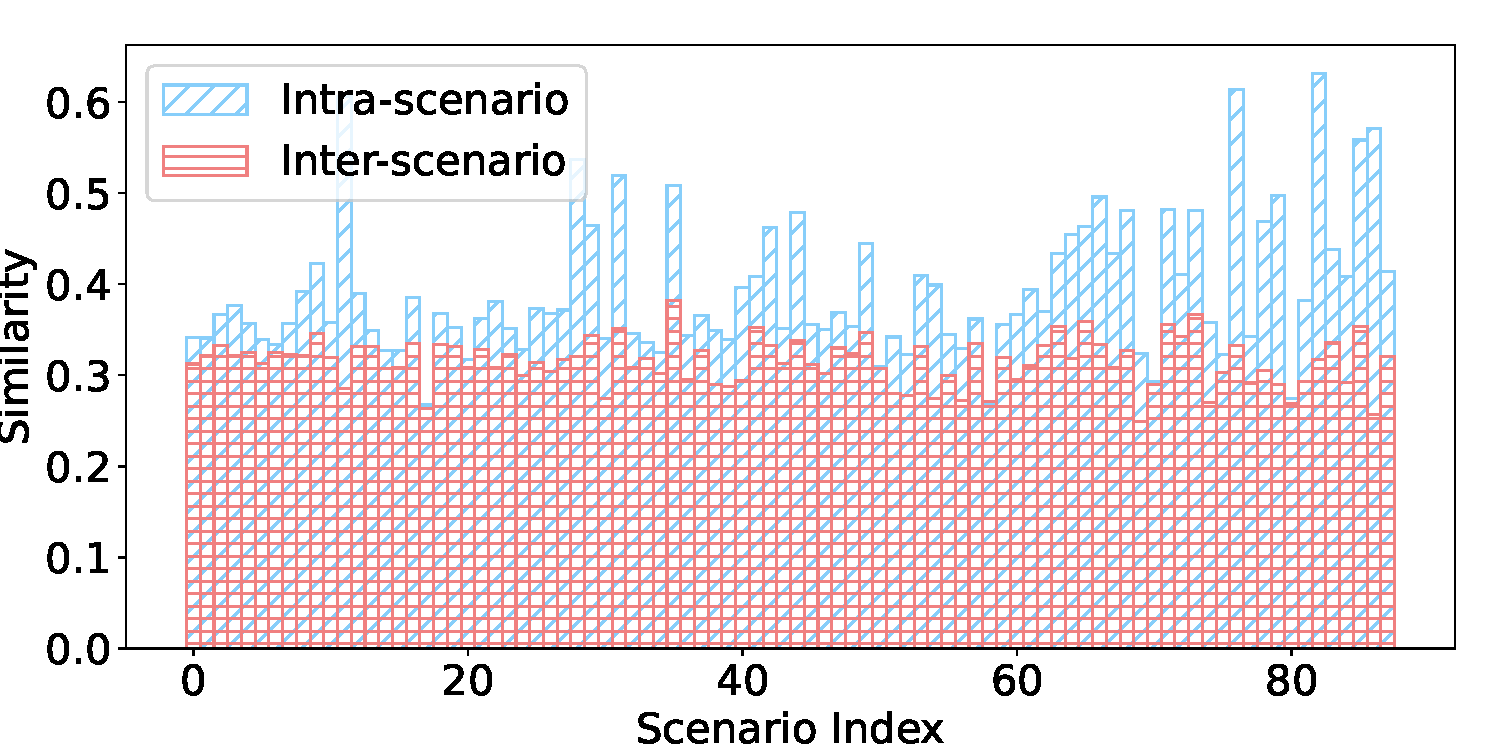
\includegraphics[width=0.8\linewidth]{chapters/egolog/figs/scenario_similarity.pdf}
    \vspace{-1em}
    \caption{Motivation for scenario understanding: 
    The similarity of embeddings for intra- and inter-scenario activities.}
    \label{fig:egolog_scenario_similarity}
    \vspace{-1em}
\end{figure}

\subsection{Scenario}
\label{subsec:scenario}
Scenario information refers to long-time activities (e.g., playing with a pet or working at home) that reflect the user's real-world behavior. Capturing such scenarios in datasets is challenging, as it requires volunteers to perform activities naturally, mimicking real-life conditions. Generally, scenario is the ensemble of multiple related and continuous activities with a realistic distribution, reflecting meaningful interactions with the environment.

To investigate the impact of scenario information on HAR, we use the Ego4D dataset~\citep{grauman2022ego4d}, which captures real-world activities through smart glasses equipped with IMU and audio sensors. The dataset provides annotations at both the window level (every 10 seconds) and the video level, represented as plain text. We treat window-level annotations as activity labels and video-level annotations as scenario labels that describe the broader setting of prolonged activities. To examine scenario properties, we use Sentence-BERT~\citep{reimers2019sentence} to generate text embeddings for activities across 91 scenarios. We then compute activity similarity both within scenarios (intra-scenario) and between scenarios (inter-scenario). Intra-scenario similarity measures the similarity of activities within the same scenario, while inter-scenario similarity compares an activity from one scenario to a randomly selected activity from a different scenario.

The results are shown in Fig.~\ref{fig:egolog_scenario_similarity}, revealing that the similarity within a scenario (intra-scenario similarity) is over 20\% higher than the similarity between different scenarios (inter-scenario similarity). This suggests that each scenario has a distinct distribution of activities. Specifically, a scenario effectively represents the user's daily log since it encompasses a longer time frame.
Additionally, we notice that the inter-scenario similarity is generally above 0.3, indicating that many basic activities (such as sitting and walking) are common across all scenarios. Therefore, it is crucial to eliminate the influence of these basic activities in scenario recognition, as they are present in every scenario.


In summary, the in-the-wild dataset shows that scenarios have distinct activity distributions, which can support scenario recognition through scenario-specific activities.


\subsection{Sound Location }
\label{subsec:embodied}
\begin{figure}
    \centering
    \begin{minipage}{0.48\linewidth}
        \centering
       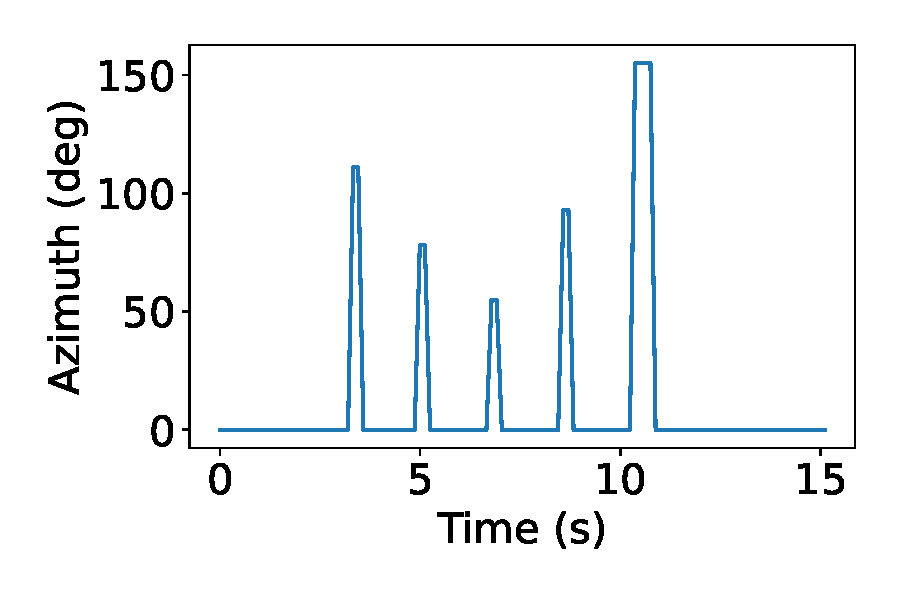
\includegraphics[width=\linewidth]{chapters/egolog/figs/baseline_result.pdf}
        \caption{Sound localization \citep{schmidt1986multiple} under motion}
        \label{fig:egolog_loc_move}
    \end{minipage}
    \hfill
    \begin{minipage}{0.48\linewidth}
        \centering
        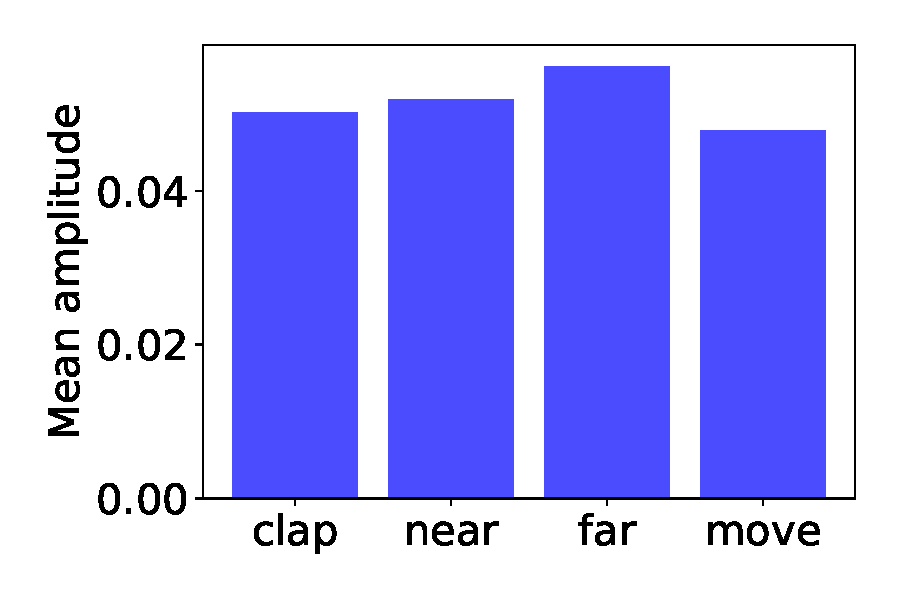
\includegraphics[width=\linewidth]{chapters/egolog/figs/amplitude.pdf}
        \caption{Sound volume may not related to distance.}
        \label{fig:egolog_amplitude}
    \end{minipage}    
    \vspace{-1em}
\end{figure}

\begin{figure}
    \centering
    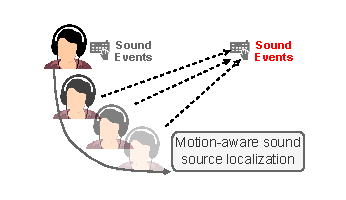
\includegraphics[width=0.75\linewidth]{chapters/egolog/figs/spatial_motivation.pdf}
    \vspace{-1em}
    \caption{Motivation for spatial understanding: estimate the distance of a sound event by motion.}
    \vspace{-1em}
    \label{fig:egolog_motivation_localization}
\end{figure}

In practice, recorded audio often includes far-field sound sources that are unrelated to the user’s activities, underscoring the importance of sound localization for effective HAR. Wearables that are consistently worn on the user’s head provide a stable and reliable position for capturing detailed ambient sound information. Additionally, modern wearables feature multi-channel recording capabilities, enhancing their spatial sensing potential.
In the following, we divide sound localization into direction and distance estimation, which we discuss as follows.

The estimation of sound direction is one of the mature, basic, but still challenging applications of a microphone array. The accuracy highly depends on the number of microphones, which is unfortunately not sufficient for most commercial devices. Considering the most common setting of stereo recording, there are mainly two problems: the deviation of direction (especially for front-back confusion) and estimation of sound distance, as illustrated in Fig. \ref{fig:egolog_motivation_localization}.
We envision that the above challenges may be solved by motion compensation. Specifically, we can aggregate the consecutive sound localization results along with the movement of the user (microphone) to refine the results or even get the distance.

To illustrate these challenges, we positioned a sound source in front of the user and used a binaural microphone with the algorithm from~\citep{schmidt1986multiple} to estimate direction of arrival, as shown in Fig.~\ref{fig:egolog_loc_move}. The user was instructed to move the body slightly and naturally. The estimate fluctuated around the true value of 90 degrees. To test whether sound volume is sufficient for differentiating near and far sources, we conducted an experiment with the sound source at different distances from the microphone. As shown in Fig.~\ref{fig:egolog_amplitude}, volume differences were not reliable across distances. The final bar in Fig.~\ref{fig:egolog_amplitude} also shows that user movement slightly affects amplitude. Multiple sound sources can further complicate volume-based distance estimation.

\subsection{Multi-modal Fusion }
\label{subsec:measure-fuse}

\begin{figure}
    \centering
     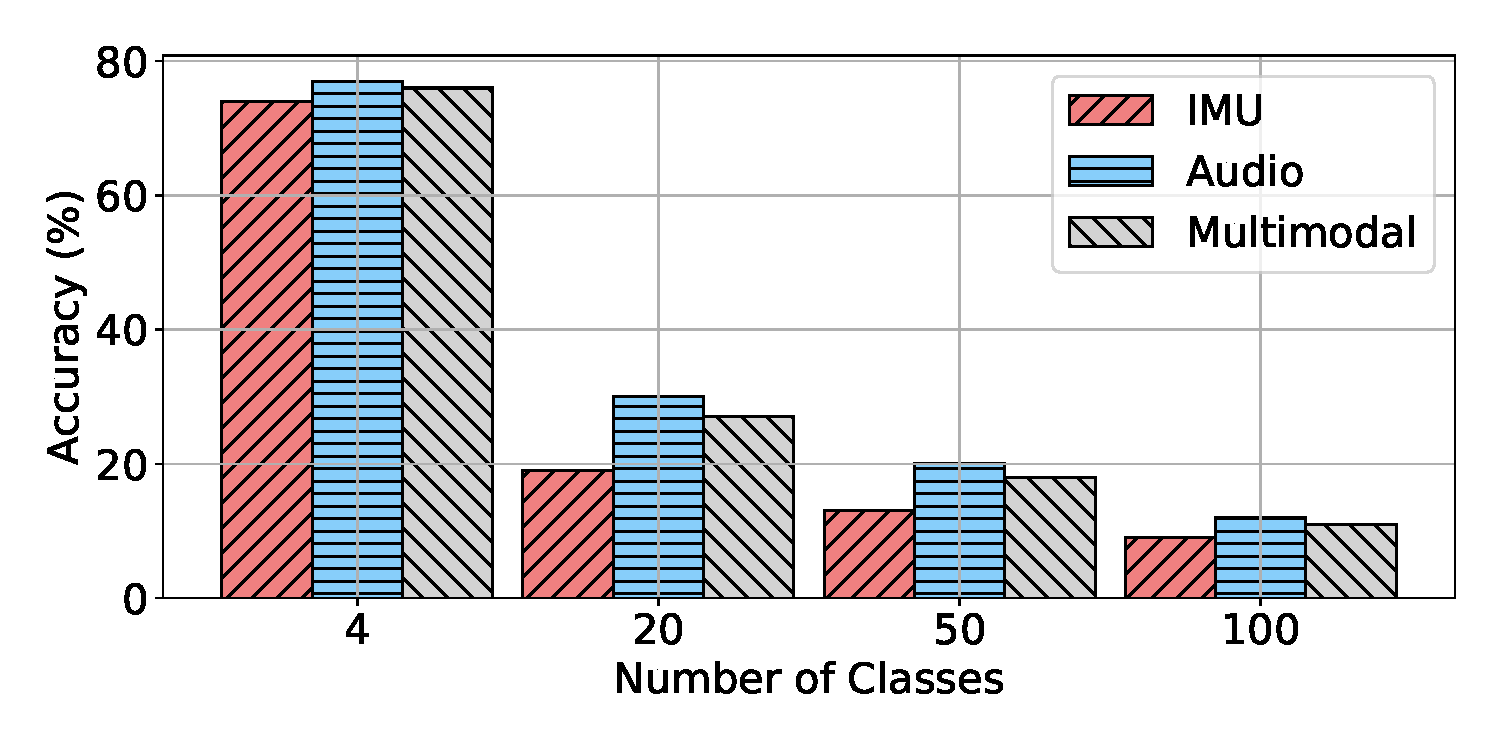
\includegraphics[width=.75\linewidth]{chapters/egolog/figs/num_class.pdf}
     \vspace{-1em}
      \caption{The performance of an existing activity recognition with different class numbers and modalities.}
    \label{fig:egolog_num_class}
    \vspace{-1em}
\end{figure}

To investigate scalability bottlenecks in activity recognition using wearables, we trained unimodal supervised models with audio and IMU data on the Ego4D episodic memory subset (200 activity classes). We used EfficientAT~\citep{schmid2023efficient} for audio and LIMU-BERT~\citep{xu2021limu} for IMU as feature extraction backbones, comparing them to a multi-modal model via late fusion. Activities were clustered into varying class numbers using Sentence BERT~\citep{reimers2019sentence} embeddings and K-Means~\citep{macqueen1967some}, following MMG-Ego4D~\citep{gong2023mmg}. Results (Fig.~\ref{fig:egolog_num_class}) show a significant performance drop as class numbers increase, indicating challenges in recognizing diverse activities with audio or IMU alone. Multimodal fusion often underperforms unimodal models, suggesting ineffective extraction of complementary features at larger scales.

\begin{figure}
    \centering
    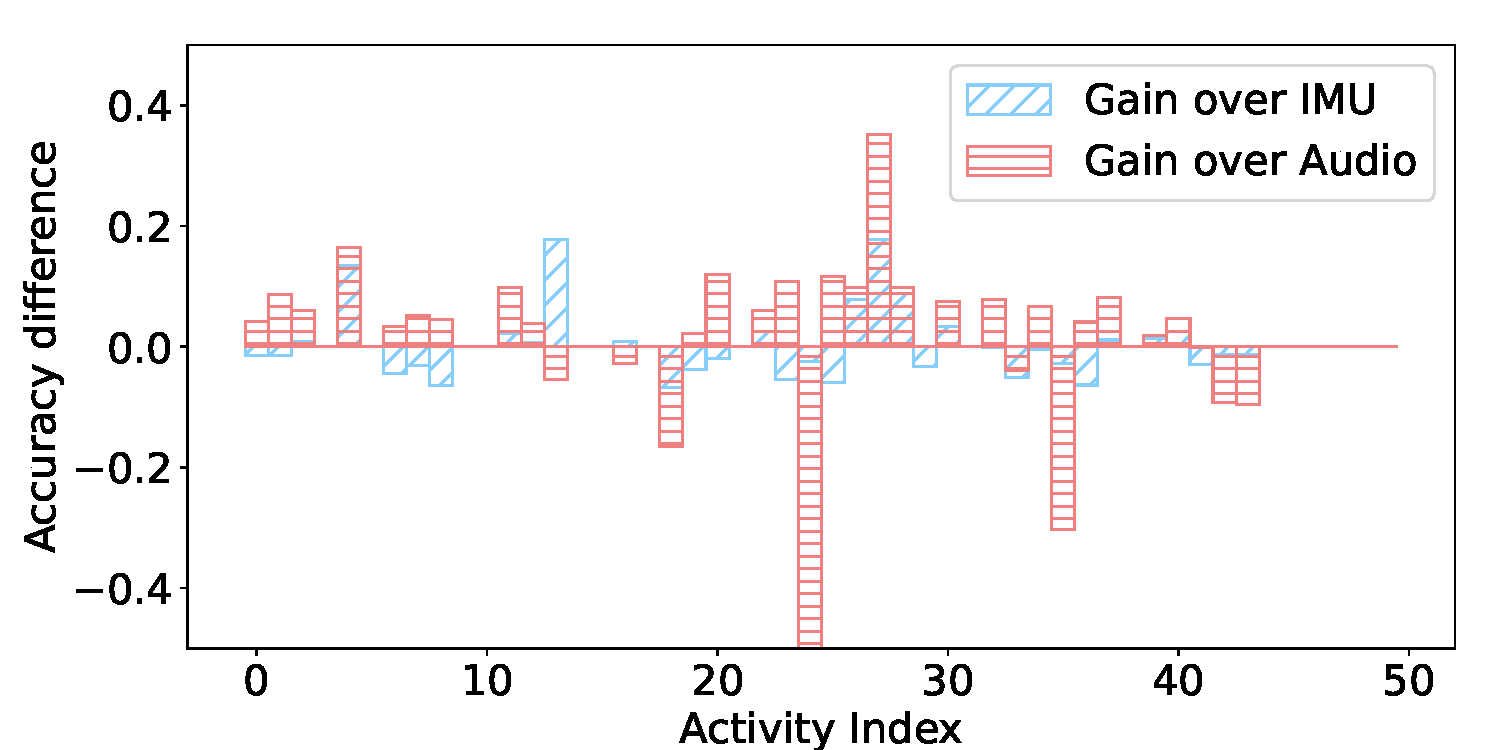
\includegraphics[width=.75\linewidth]{chapters/egolog/figs/activity_diff.pdf}
    \vspace{-1em}
    \caption{Performance gain from multi-modal fusion.}
    \label{fig:egolog_acc_gap}
    \vspace{-1em}
\end{figure}

Previous work~\citep{mollyn2022samosa} demonstrates that multi-modal learning can outperform the unimodal model due to the complementary nature of each other.
However, this finding does not apply to all cases. Another study~\citep{gong2023mmg} finds that multimodal learning with audio and IMU on Ego4D can perform worse than single-modality solutions. To investigate this result, we compared the accuracy of multimodal and unimodal models for each class, as shown in Fig.~\ref{fig:egolog_acc_gap}. The benefits of multimodal fusion fluctuate across both modalities, indicating that supervised multimodal learning cannot automatically select the appropriate modality for each activity.


To investigate whether LLMs can alleviate this problem, we evaluate ImageBind-LLM~\citep{han2023imagebind}, which converts both modalities into features and prepends them to text embeddings. We instruct the model with the prompt: ``<sensor> According to the audio and IMU reading on the earphone of the user, what is the activity of the user?'', where <sensor> denotes the inserted sensor features. Since LLM outputs can be random, we also constrain the prompt to one of the candidate activities. To reduce complexity, we select the top 30 activities from the Ego4D episodic memory subset. ImageBind-LLM achieves BERT-score precision, recall, and F1 score of 0.04, 0.07, and 0.05, respectively. Because this performance is low, we inspect the outputs and find that the LLM may not fully understand the multimodal fusion task.
We further test whether fine-tuning can address this problem by training an adapter~\citep{zhang2023llamaadapter} for ImageBind-LLM. The adapted LLM achieves BERT-score precision, recall, and F1 score of 0.47, 0.46, and 0.47, respectively. Although fine-tuning improves performance, the result remains below the level needed for practical use.
